\subsubsection{Contract Creation}
\label{sec:contract-creation}
The contract creation is the act by which a new contract is deployed on the
system. It can be triggered either by a transaction or during the execution of
an existing contract. In the remainder of this section, we use the neutral term
\textit{sender} to refer to the entity who starts the contract creation. In the
first case the sender corresponds to the transaction initiator and in the
second case it corresponds to the address of the contract that is executing.

\begin{figure}
	\begin{center}
		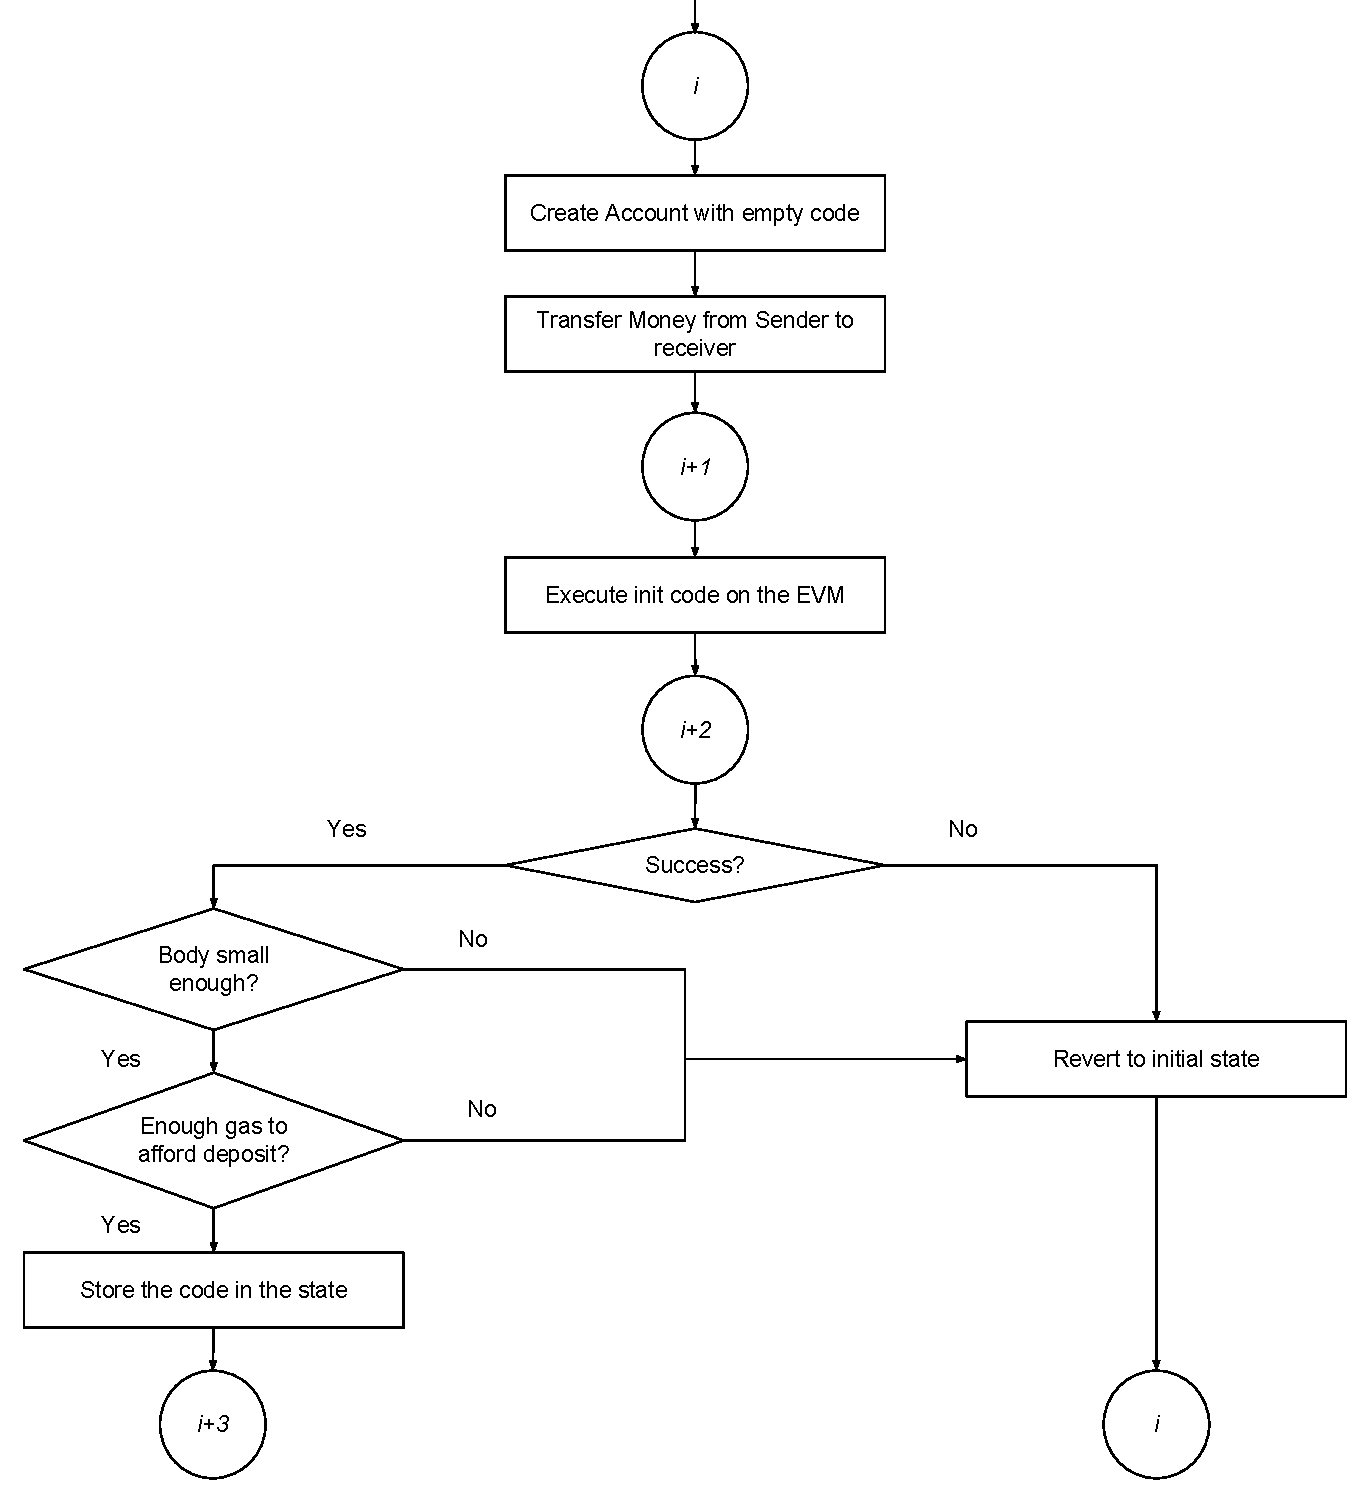
\includegraphics[width=\textwidth]{./res/img/contract-creation.pdf}
	\end{center}
	\caption{The steps of the contract creation algorithm.}
	\label{fig:contract-creation}
\end{figure}

The steps of the algorithm and the state transition are depicted in
\autoref{fig:contract-creation}. The circles represent the different states.
Firstly, the 160-bit identifier for the contract account is determined as
function of the sender's address and its nonce. The value specified in the
contract
creation is transferred from the sender to the brand new contract account.
Afterward, the \textbf{init} code is executed on the Ethereum Virtual Machine.
This  piece of code initiate the storage of the contract account and returns the
\textbf{body}, i.e. the contract code that will persist on the account state. If
during the execution an out-of-gas exception occurred, the state is reverted to
the initial state as if the contract creation did not take place. If the
execution of the init code completed successfully, the creator must pay an
amount of gas proportional to the size of the \textbf{body}, because it must be
stored by all the full nodes. If the gas remained after the execution is not
enough to afford this cost or the body of the contract code is too big, the
state is reverted~\cite{wood2018ethereum}. If all the whole procedure succeed,
the hash of the body is saved on the contract account state. Usually, the
implementations use this hash as a key for the contract code, as showed in
\autoref{fig:world-state}.

